\newpage
\section{Búsqueda de estudios}

Esta etapa comprendió las siguientes secciones:
\begin{enumerate}
	\item Estrategia de búsqueda, ya sea independiente o combinada;
	\item Identificación general de estudios;
	\item Revisión de estudio; y finalmente,
	\item Selección de estudios para incluir en el \ac{SMS}.
\end{enumerate}


\subsection{Estrategia de búsqueda}\label{subsec:estrategia-busqueda}

La estrategia de búsqueda empleada en este estudio combinó consultas estructuradas en bases de datos científicas con la técnica de búsqueda en bola de nieve (\textit{snowballing}). Esta integración metodológica permitió ampliar el alcance del proceso de identificación de literatura relevante, favoreciendo la recuperación de estudios adicionales a partir de las referencias bibliográficas y citaciones de los trabajos inicialmente seleccionados. Como resultado, fue posible identificar investigaciones de interés que podrían no haber sido localizadas mediante la aplicación exclusiva de estrategias de búsqueda tradicionales, fortaleciendo así la exhaustividad y cobertura del mapeo sistemático.


\subsection{Búsqueda en bases de datos}\label{subsec:busqueda-bases-datos}

Para la realización del \ac{SMS}, se seleccionaron las bases de datos Web of Science, IEEE Xplore, Springer, ScienceDirect y Taylor \& Francis. La elección de estas fuentes se fundamentó en su reconocida relevancia dentro de la comunidad científica, así como en la amplitud y calidad de la literatura que indexa en el área de investigación objeto de estudio. Adicionalmente, su disponibilidad y cobertura temática permitieron garantizar el acceso a publicaciones científicas actualizadas y pertinentes, contribuyendo a la rigurosidad y confiabilidad del proceso de búsqueda y selección de la evidencia científica.


\subsubsection{Identificación de estudios mediante búsqueda en bases de datos}\label{subsubsec:identificacion-estudios}

En esta etapa fue necesario definir un marco de referencia que facilitara la identificación y selección de las palabras clave más adecuadas para la construcción de la cadena de búsqueda empleada en las bases de datos seleccionadas. Con este propósito, se utilizó el modelo \ac{PICOC} como guía metodológica para estructurar y delimitar los términos de búsqueda relacionados con el objeto de estudio. La aplicación de este modelo permitió sistematizar el proceso de definición de palabras clave, favoreciendo la consistencia y trazabilidad de la estrategia de búsqueda. El resultado de este procedimiento se presenta en las \autoref{tab:modelo-picoc} y \autoref{tab:palabras-clave-picoc}.

\begin{table}[H]
	\centering
	\caption{Modelo \acs{PICOC}}
	\label{tab:modelo-picoc}

	\renewcommand{\arraystretch}{1.2}
	\fontsize{9pt}{10pt}\selectfont

	\begin{tabularx}{\textwidth}{|c|X|}
		\hline
		\tableheader
		\textbf{Componente} &
		\textbf{Descripción}
		\\
		\hline
		Población           &
		Estudios relacionados con los servicios de directorio
		\\
		\hline
		Intervención        &
		Observación y tabulación.
		\\
		\hline
		Comparación         &
		Identificación de características técnicas y arquitectónicas reportadas en las herramientas tecnológicas.
		\\
		\hline
		Salidas             &
		Conjunto de herramientas tecnológicas de servicios de directorio de código abierto y sus características técnicas y arquitectónicas.
		\\
		\hline
		Contexto            &
		Gestión institucional, servicios de directorio, seguridad, autenticación e identidad.
		\\
		\hline
	\end{tabularx}
\end{table}

\begin{table}[H]
	\centering
	\caption{Palabras clave identificadas usando el modelo PICOC}
	\label{tab:palabras-clave-picoc}

	\renewcommand{\arraystretch}{1.2}
	\fontsize{9pt}{10pt}\selectfont

	\begin{tabularx}{\textwidth}{|c|X|}
		\hline
		\textbf{Categoría PICOC}         &
		\textbf{Palabras clave}
		\\
		\hline
		\textbf{Población}               &
		Directory services, Identity management systems, Authentication systems, Authorization systems, LDAP systems
		\\
		\hline
		\textbf{Intervención}            &
		Open source directory service, Free software, OpenLDAP, Open source identity management, LDAP implementation
		\\
		\hline
		\textbf{Criterios de aceptación} &
		Proprietary directory service, Commercial solutions, Active Directory
		\\
		\hline
		\textbf{Salidas}                 &
		Technical characteristics, Software architecture, Scalability, Security, Interoperability
		\\
		\hline
		\textbf{Contexto}                &
		Distributed infrastructure, Research infrastructure, Academic environment
		\\
		\hline
	\end{tabularx}
\end{table}


Los términos de búsqueda identificados a partir del modelo \ac{PICOC} y presentados en la \autoref{tab:palabras-clave-picoc} fueron complementados mediante la incorporación de sinónimos y conceptos relacionados, con el fin de ampliar la cobertura y sensibilidad del proceso de recuperación de estudios. El conjunto resultante de términos se muestra en la \autoref{tab:palabras-clave}. Estos términos constituyeron la base para la cadena de búsqueda utilizada en cada una de las bases de datos seleccionadas.

\begin{table}[H]
	\centering
	\caption{Palabras clave para la búsqueda en bases de datos}
	\label{tab:palabras-clave}

	\renewcommand{\arraystretch}{1.2}
	\fontsize{9pt}{10pt}\selectfont

	\begin{tabularx}{\textwidth}{|c|X|}
		\hline
		\tableheader
		\textbf{Palabra clave}     &
		\textbf{Sinónimos}
		\\
		\hline
		\textbf{Directory service} &
		Directory services, Network directory service, User directory
		\\
		\hline
		\textbf{LDAP}              &
		Lightweight Directory Access Protocol, LDAP-based system, LDAP directory service
		\\
		\hline
	\end{tabularx}
\end{table}


Con el objetivo de filtrar los resultados obtenidos y centrar el análisis en estudios relevantes para la investigación, se definieron criterios de inclusión y exclusión, los cuales se presentan en la \autoref{tab:criterios-inclusion-exclusion}. Estos criterios orientaron el proceso de selección de estudios, permitiendo identificar aquellos trabajos alineados con objetivos del \ac{SMS} y descartar aquellos que no contribuían de manera significativa a la respuesta de las preguntas de investigación ni al desarrollo del análisis.

\begin{table}[H]
	\centering
	\caption{Criterios de inclusión y exclusión}
	\label{tab:criterios-inclusion-exclusion}

	\renewcommand{\arraystretch}{1.2}
	\fontsize{9pt}{10pt}\selectfont

	\begin{tabularx}{\textwidth}{|c|X|X|}
		\hline
		\textbf{Categoría}                                                         &
		\textbf{Inclusión}                                                         &
		\textbf{Exclusión}
		\\
		\hline
		Campos                                                                     &
		Resumen, título y palabras clave.                                          &
		Documento completo
		\\
		\hline
		Tipo de publicación                                                        &
		Artículos, libros, capítulos de libros y actas de congresos.               &
		Tesis
		\\
		\hline
		Área/Disciplina                                                            &
		Administración, ciencias de la computación y tecnología de la información. &
		Áreas no relacionadas con la administración, las ciencias de la computación, las tecnologías de la información y la gestión.
		\\
		\hline
		Periodo                                                                    &
		Entre 2020 y 2026                                                          &
		Menos de 2020
		\\
		\hline
		Idioma                                                                     &
		Inglés y Español                                                           &
		---
		\\
		\hline
	\end{tabularx}
\end{table}



\subsubsection{Búsqueda en bases de datos}\label{par:busqueda-bases-datos}

La cadena de búsqueda correspondiente a cada una de las bases de datos seleccionadas se presenta en la \autoref{tab:cadena-busqueda}.

\begin{table}[H]
	\centering
	\caption{Cadena de búsqueda}
	\label{tab:cadena-busqueda}

	\renewcommand{\arraystretch}{1.2}
	\fontsize{9pt}{10pt}\selectfont

	\begin{tabularx}{\textwidth}{|X|}
		\hline
		\tableheader
		\textbf{Cadena de búsqueda} \\
		\hline
		(``Directory service'' OR ``Directory services'' OR ``User directory'') AND (``LDAP'' OR ``Lightweight Directory Access Protocol'' OR ``LDAP-based system'')
		\\
		\hline
	\end{tabularx}
\end{table}




\subsubsection{Métricas de la búsqueda sin criterios de inclusión/exclusión}\label{subsubsec:resumen-busqueda}

La \autoref{tab:bases-sin-exclusion} presenta la cantidad de publicaciones recuperadas en las bases de datos consultadas durante la búsqueda inicial, previa a la aplicación de los criterios de inclusión y exclusión. En esta etapa se identificaron un total de 1720 registros, distribuidos entre IEEE Xplore (39), \ac{WOS} (10), Springer (1019), Taylor \& Francis (38) y ScienceDirect (614). El detalle de esta búsqueda preliminar se presenta en el apéndice \ref{sec:busqueda-sin-criterios}.

\begin{table}[H]
	\centering
	\caption{Resultados de la búsqueda sin exclusión}
	\label{tab:bases-sin-exclusion}

	\renewcommand{\arraystretch}{1.2}
	\fontsize{9pt}{10pt}\selectfont

	\begin{tabularx}{\textwidth}{|X|c|c|c|>{\centering\arraybackslash}m{1.5cm}|c|c|}
		\hline
		\tableheader
		\textbf{Criterios}                               &
		\textbf{IEEE}                                    &
		\textbf{WOS}                                     &
		\textbf{Springer}                                &
		\textbf{Taylor \& Francis}                       &
		\textbf{ScienceDirect}                           &

		\textbf{Total}
		\\
		\hline
		Cadena de búsqueda con palabras clave únicamente &
		39                                               &
		10                                               &
		1019                                             &
		38                                               &
		614                                              &
		1720
		\\
		\hline
		Contribución porcentual                          &
		2,27\%                                           &
		0,58 \%                                          &
		59,24\%                                          &
		2,21\%                                           &
		35,70\%                                          &
		100\%
		\\
		\hline
	\end{tabularx}
\end{table}



\subsubsection{Métricas de la búsqueda con criterios de inclusión/exclusión}\label{subsec:resumen-busqueda-citerios}

Esta búsqueda aplicó los criterios de inclusión y exclusión previamente definidos. Si bien se utilizó la misma cadena de búsqueda, esta etapa se diferencia por la aplicación de filtros específicos en cada base de datos. Las evidencias correspondientes a este proceso pueden consultarse en el apéndice~\ref{sec:busqueda-con-criterios}.

La \autoref{tab:bases-con-exclusion} presenta los resultados obtenidos tras la aplicación de los criterios de inclusión y exclusión. En contraste con la búsqueda inicial, en esta fase los filtros aplicados redujeron de manera significativa la cantidad de publicaciones recuperadas. En total, se identificaron 159 documentos, distribuidos de la siguiente manera: IEEE Xplore (3), \ac{WOS} (1), Springer (132), Taylor \& Francis (1) y ScienceDirect (22).

\begin{table}[H]
	\centering
	\caption{Resultados de la búsqueda con criterios de exclusión}
	\label{tab:bases-con-exclusion}

	\renewcommand{\arraystretch}{1.2}
	\fontsize{9pt}{10pt}\selectfont

	\begin{tabularx}{\textwidth}{|X|c|c|c|>{\centering\arraybackslash}m{1.5cm}|c|c|}
		\hline
		\tableheader
		\textbf{Criterios}                                        &
		\textbf{IEEE}                                             &
		\textbf{WOS}                                              &
		\textbf{Springer}                                         &
		\textbf{Taylor \& Francis}                                &
		\textbf{ScienceDirect}                                    &

		\textbf{Total}
		\\
		\hline
		Cadena de búsqueda con criterios de inclusión y exclusión &
		3                                                         &
		1                                                         &
		132                                                       &
		1                                                         &
		22                                                        &
		159
		\\
		\hline
		Contribución porcentual                                   &
		1,89\%                                                    &
		0,63 \%                                                   &
		83,01\%                                                   &
		0,63\%                                                    &
		13,84\%                                                   &
		100\%
		\\
		\hline
	\end{tabularx}
\end{table}


El resultado del proceso de búsqueda en bases de datos puede observarse en la \autoref{fig:resumen-busqueda-bases}. Como se aprecia, tras la aplicación de los criterios de inclusión y exclusión se descartaron 1561 estudios, lo que representa una reducción del 90.76\% respecto a los resultados de la búsqueda inicial.

\begin{figure}[H]
	\centering
	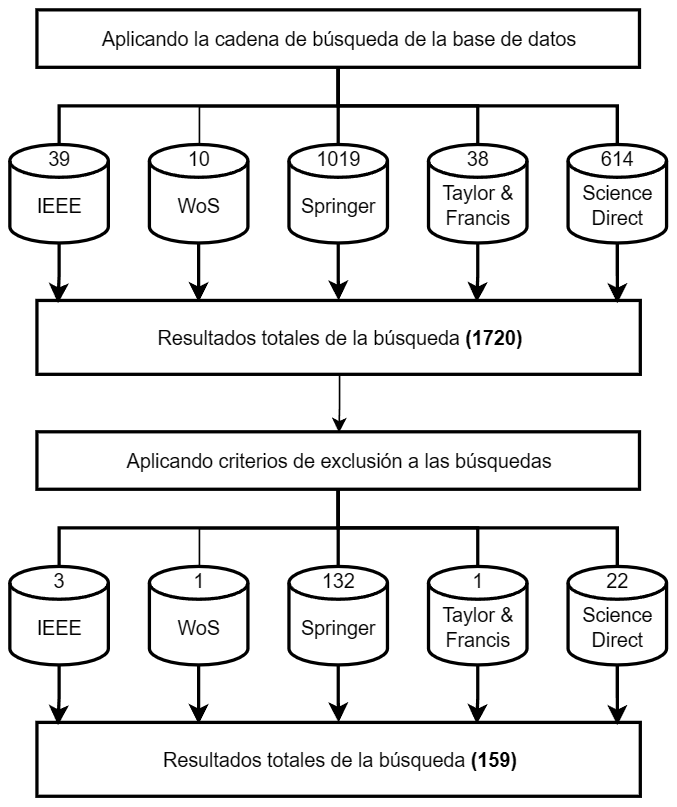
\includegraphics[width=0.7\textwidth]{mainmatter/II-desarrollo-metodologico/sms/imagenes/resumen-busqueda-bases.png}
	\caption{Diagrama resumen del proceso de búsqueda en bases de datos}
	\label{fig:resumen-busqueda-bases}
\end{figure}
